%!TEX root = ../../report.tex
\section{Mapping with Location noise}

\subsection{Monte Carlo localization}
The robot estimates its localization with the an adaption of the ROS implementation \cite{ros_amcl} of the adaptive monte carlo localization(AMCL) \cite{Thrun200199}. It uses a particle filter to track the robot's pose in a known map. 
The estimated uncertainty on the localization is described with a covariance matrix. The covariance matrices for some of the locations the robot visited during navigation in an industrial environment is visualized as contour plots around the robots position(green) in figure \ref{fig:amcl_covariance}. 
The figure shows that the estimated standard deviation on the positional error generally is around $10cm$. Around the corner the estimated standard deviation however increase to more than twice that. This is reasonably since the map used by AMCL for scan matching was wrong in the top left corner of figure \ref{fig:amcl_covariance}. The estimated angular error also doubles when the robot reaches the corner.
In figure \ref{fig:simulated_small_world} the simulated world is shown. The corresponding map used by AMCL to estimate the robot pose is shown in \ref{fig:simulated_small_amcl_map}.
It is clearly visible from the maps that AMCL was missing information about the world. The lack of correspondence between the maps causes the covariance of the pose estimate to increase.
Marked on each figure are the path the robot drove through the world, both the estimated and the true path.
A ROS bag was created of the run in order to ensure all methods was given the same input. 

\begin{figure}
	\centering
	\begin{subfigure}[b]{0.45\textwidth}
		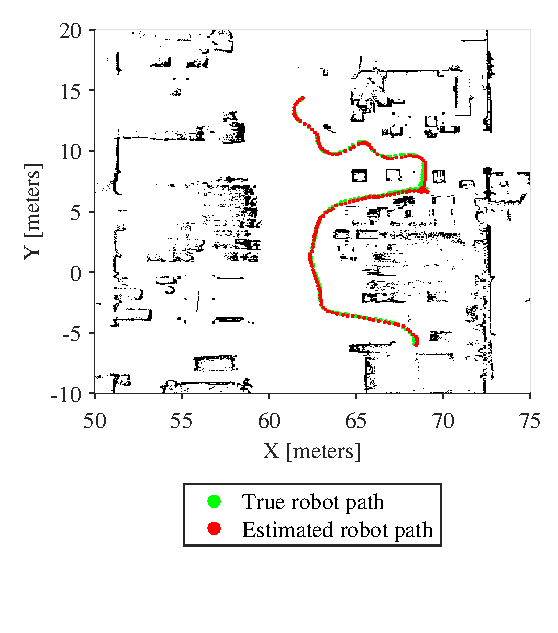
\includegraphics[width=\textwidth]{figures/static_mapping/map_with_poses}
		\caption{World represenation}
		\label{fig:simulated_small_world}
	\end{subfigure}
	~ %add desired spacing between images, e. g. ~, \quad, \qquad, \hfill etc. 
	%(or a blank line to force the subfigure onto a new line)
	\begin{subfigure}[b]{0.45\textwidth}
		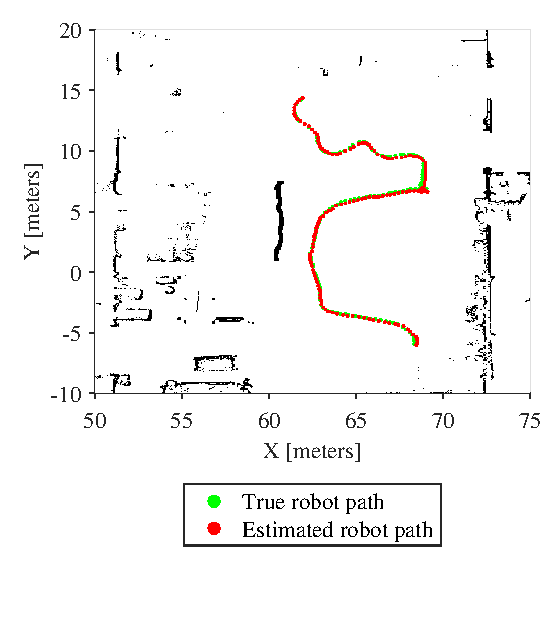
\includegraphics[width=\textwidth]{figures/static_mapping/amcl_map_with_poses}
		\caption{Map used by AMCL}
		\label{fig:simulated_small_amcl_map}
	\end{subfigure}
	\caption{Simulation of a MIR robot moving with imprecise location.}
	\label{fig:test_map_setup}
\end{figure}


\begin{figure}[tbph]
\centering
	\begin{subfigure}[b]{0.75\textwidth}
		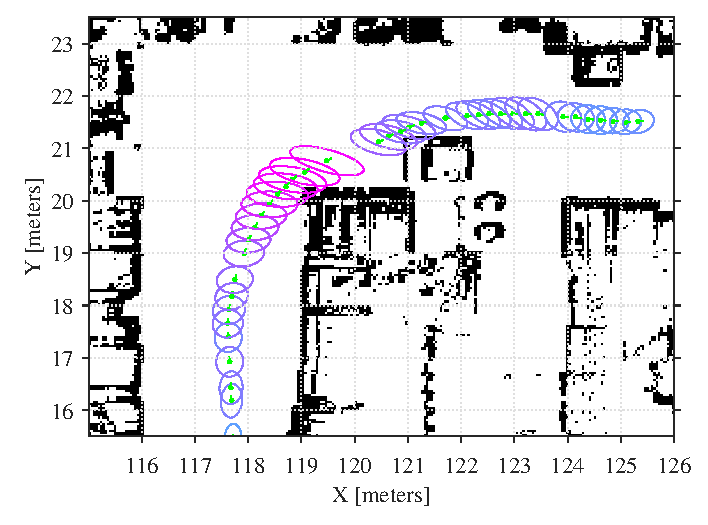
\includegraphics[scale=1.0]{figures/static_mapping/amcl_covariance}		
		\label{fig:amcl_covariance}
	\end{subfigure}
	~ %add desired spacing between images, e. g. ~, \quad, \qquad, \hfill etc. 
	%(or a blank line to force the subfigure onto a new line)
	\begin{subfigure}[b]{0.2\textwidth}
		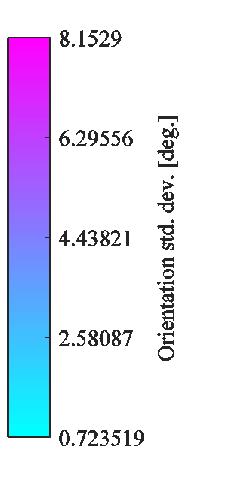
\includegraphics[scale=1.0]{figures/static_mapping/amcl_covariance_bar}
		\label{fig:amcl_covariance_bar}
	\end{subfigure}
	\caption{Covariances estimated by AMCL in an industrial environment shown with contours marking one standard deviation around the robot's estimated pose(green).}
\end{figure}

\subsection{Non-ideal Inverse Sensor Model}
From hector

\subsection{Monte Carlo Integration Inverse Sensor Model}
\label{monte_carlo_sensor Model}
The monte carlo integration inverse sensor Model proposed by Joubert, Brink and Herbst \cite{Joubert2014},  uses the fact that particles used in Monte Carlo Localization with their likelihood weights approximates the robots uncertainty. 
It works by ray-tracing the sensor measurements with a weighted ordinary inverse sensor model from the particles' poses instead of the estimated pose. 
Equation \ref{eq:monte_carlo_sensor_model} shows how a log-odds occupancy cell is updated with the right most term consistent of a weighted sum of inverse sensor models for $K$ particles.

\begin{equation}
log \frac{p(m_i|z_{1:t})}{1-p(m_i|z_{1:t})} = log \frac{p(m_i|z_{1:t-1})}{1-p(m_i|z_{1:t-1})} + \sum_{i=1}^{K} w_t^i log \frac{ p(m_i | z_t^i) }{ 1 - p(m_i | z_t^i) }
\label{eq:monte_carlo_sensor_model}
\end{equation}

It can be computational expensive to ray-tracing the often several hundred measurements every tenth of a second from each of the often several hundreds of particles.
To avoid this only the $K$ top most weighted particles are used.% Jeg tror ikke de skal omvægtes

Figure \ref{fig:particle_sensor} shows how most of the ray-traced inverse sensor models results in similar look maps along the rays. 
It is represented as a heat map where the black is low probability for occupancy and the white is high. 
It can however be seen that some of the particles are orientated significantly different from the rest. 
See how the model have built a map where there are a small probability for occupancy along the rays with similar distance by rotated around the robot's pose (red square). This lack of concurrence ray-traced lines when the particles are misaligned leads to lower confidence in the measurements when the estimated particles are spread out. The degree of this increases with a further spread of particles.

\begin{figure}
	\centering
	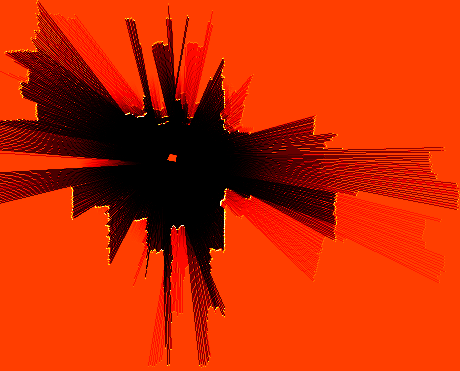
\includegraphics[width=0.7\linewidth]{figures/static_mapping/particle_sensor}
	\caption{Example map with few LiDar measurements from the five highest (re-weighted/wrong) weighted particles.}
	\label{fig:particle_sensor}
\end{figure}

\subsection{Cone based model}
An attempt to represent the pose uncertainty in the static mapping is model based on a sonar-like cone. The idea is to represent the uncertainty of origin position and angle of each laser ray with a broad centered cone. 
This cone, which can be seen in figure  \ref{fig:cone_with_noise_top}, consist of three areas. These are the center, the left side cone and right side cone. As the model is based on a sonar cone model [REFERENCE TO SONARCONE], the values of a cell is determined by the distance from the origin and the angle to the straight line to the target. The changes from the original sonar model is the center section which splits the two cone halves. 

The angle \(\theta\) is equal to the standard deviation of the orientation estimate. 
The width of the center area, w, is determined by the sum of the projection of the standard deviation in the x and y directions perpendicular to the ray direction. 

The value of a cell is determined by the distance from the origin line. 
[For instance the value at the point p in figure \ref{fig:cone_with_noise_top} is determined by the the distance l.] 
The width, m, of the marking cone is determined by the position error projected onto the ray.

It is possible to add a weight to cell value. This weight is calculated
\begin{equation}
\label{eq:cone-weight}
weigth = 
\begin{cases}
1 - ( 2 \cdot \theta \cdot l + w), & \text{if } 2 \cdot \theta \cdot l + w < 1\\
0, & \text{otherwise}
\end{cases}
\end{equation}

\begin{figure}
	\centering
	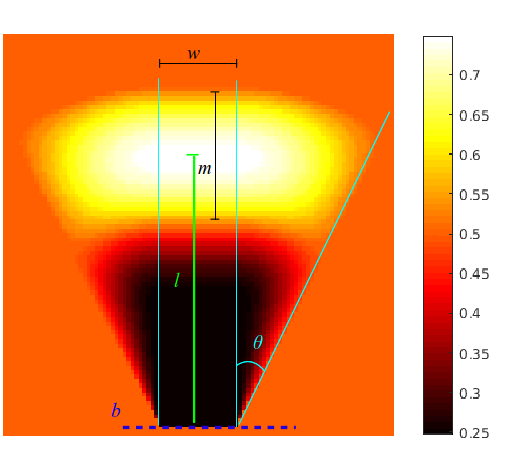
\includegraphics[width=\textwidth]{figures/static_mapping/cone_noise_top}
	\caption{Cone representing pose noise}
	\label{fig:cone_with_noise_top}
\end{figure}



\subsection{Comparison of Inverse Sensor Models}
In order to compare the various mapping methods a metric for determining the accuracy of a map. One of the methods for comparing to occupancy maps is the map score, first proposed in [REFERENCE TO ELFES MAPSCORE]. The score is calculated as the squared error between the occupancy for each cell in two maps, as seen in equation \ref{eq:MapScore}.

\begin{equation}
\label{eq:MapScore}
Score = \sum_{n=0}^{N} (m_{n} - o_{n})^2
\end{equation}

N is all cells in the maps m and o. 
This gives a simple result that indicates how alike two maps are. 
However, as most maps contains vastly more free space than occupied space this might skew the result. 
A map can receive a higher score for asserting strong statements about free cells but not mapping obstacles very accurate. 
As the obstacles are vital parts of the map this is not desired. 
To overcome this it is suggested to only use cells where either one of the maps have an occupied probability higher than \(0.5\) [REFERENCE TO EVAL OF MAP METHODOLEGIES]. 
If the MapScore is to be used to evaluate a mapping algorithm between different maps, it is necessary to normalize the score with the number of cells in the map tested. 

Figure \ref{fig:score_comparison} shows the scores for different sensor models and methods. 

\begin{figure}
	\label{fig:score_comparison}
	\begin{subfigure}[b]{0.45\textwidth}
		\centering
		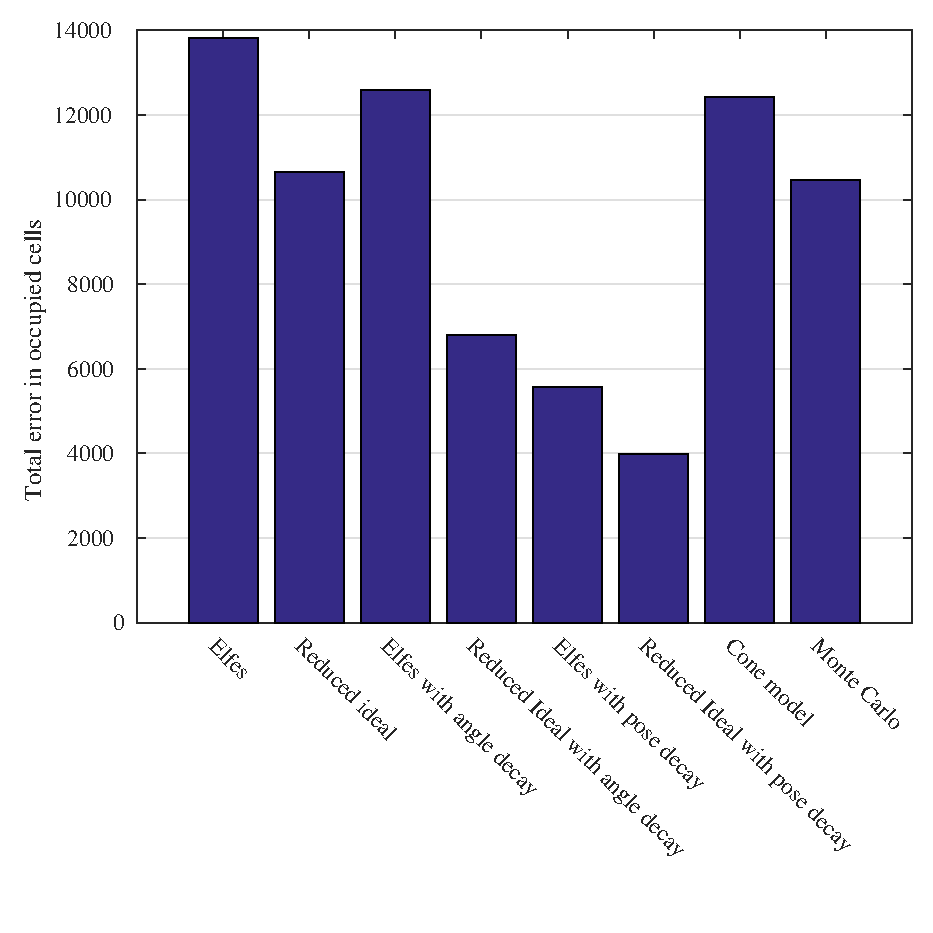
\includegraphics[scale=1]{figures/static_mapping/comparison_obstacle_error}
		\caption{MapScore - obstacles only}
		\label{fig:comparison_obstacle_error}
	\end{subfigure}
	\begin{subfigure}[b]{0.45\textwidth}
		\centering
		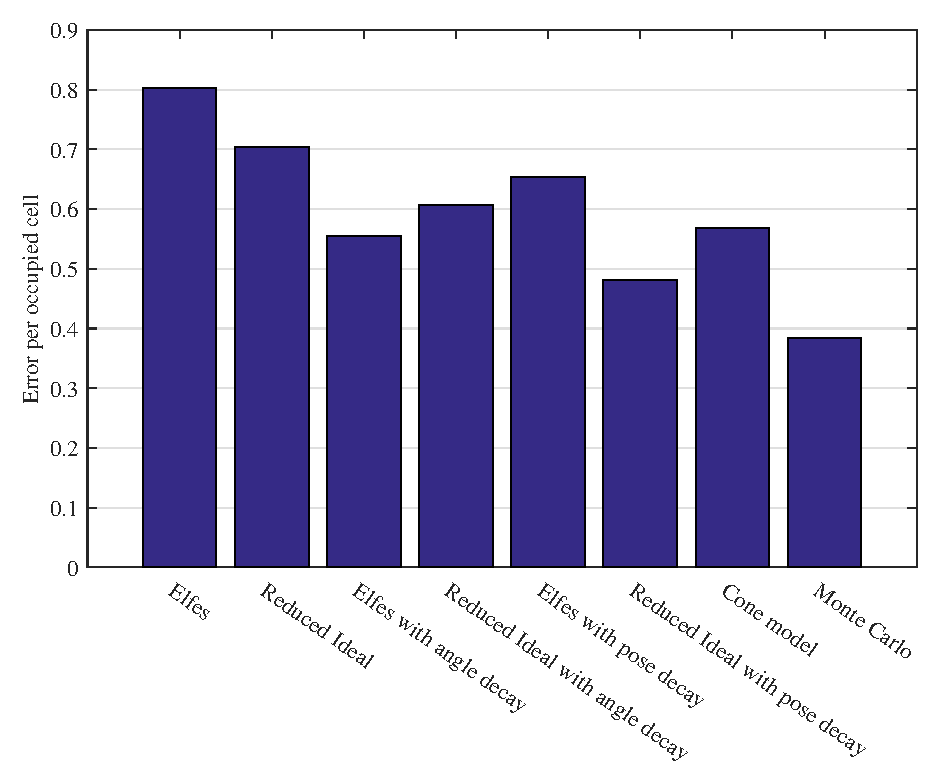
\includegraphics[scale=1]{figures/static_mapping/comparison_obstacle_error_per_cell}
		\caption{MapScore - normalized by number of obstacle cells}
		\label{fig:comparison_obstacle_error_per_cell}
	\end{subfigure}
	\caption{MapScores for different methods}
\end{figure}